\documentclass[11pt]{article}
\usepackage[estonian]{babel}
\usepackage[utf8]{inputenc}
\usepackage{enumerate}
\usepackage{graphicx}

\title{\textbf{GapBammon}}
\author{Madis Pink\\
		Mikk Pavelson\\
		Uku Loskit\\
		Lauris Kruusamäe}
\date{}
\begin{document}

\maketitle

\newpage
\section{Project Schedule}
\textbf{08.10}
\begin{enumerate}[1]
\item Write schedule
\item Acquire domain knowledge (backgammon rules and playing experience)
\item Storyboard
\item Write project requirements and aims
\item Infrastructure setup
\end{enumerate}
\textbf{09.10}
\begin{enumerate}[1]
\item Create class diagram
\item Write code
\end{enumerate}
\textbf{11.10}
\begin{enumerate}[1]
\item Write code
\item Test
\item Write repository / code outline
\item Documentation cleanup
\end{enumerate}
\textbf{12.10}
\begin{enumerate}[1]
\item Release
\item Submit assignment
\end{enumerate}

\newpage
\section{Storyboard}

\textbf{Background}

John and Miles are long-time friends and want to play backgammon together. Unfortunately they both live in different parts of the city and have access to a teletype terminal. So, they turn to GapBammon...

\begin{enumerate}[I]
\item John and Miles start a game of CLI backgammon by running a command in a terminal. John inputs his name first and becomes player1, Miles is upset because he is forced to be player2. Miles enters his name.
	
GapBammon rolls the dice for both players, John rolls a 6, Miles rolls a measly 2. This means that John is better again and gets to go first. 

\begin{figure}[!h]
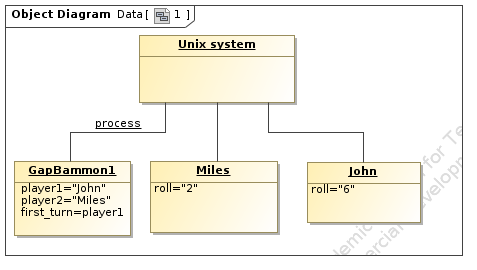
\includegraphics[scale=0.8]{1.png}
\end{figure}
\newpage
\item Miles and John have started the game. John needs to make a move against Miles. A backgammon board is displayed on the terminal screen (ASCII art). The game rolls dice for John with the outcome of 4 and 6. Now John can see a list of all available moves and select two of them consecutively to finish his turn. And so he does. The board is printed again to reflect the new game state.

\begin{figure}[!h]
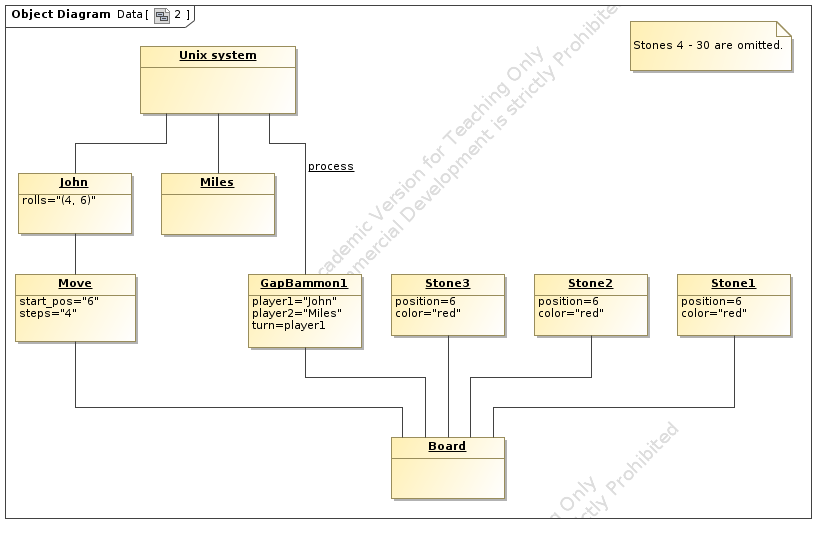
\includegraphics[scale=0.5]{2.png}
\end{figure}
\newpage
\item 30 minutes of unearthly action follow. Suddenly, Miles is ahead and needs to make a final move. All but one of his stones have found their way into the basket. The game rolls doubles (two sixes) for Miles, which he easily turns into a win. The game ends and declares Miles the victor. 
John ragequits.

\begin{figure}[!h]
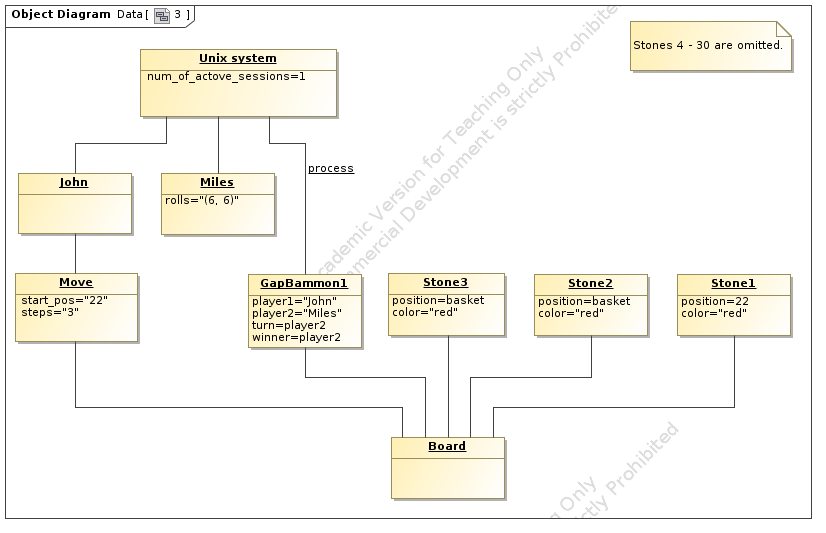
\includegraphics[scale=0.5]{3.png}
\end{figure}
\end{enumerate}
\newpage

\section{Class Model}
\begin{figure}[!h]
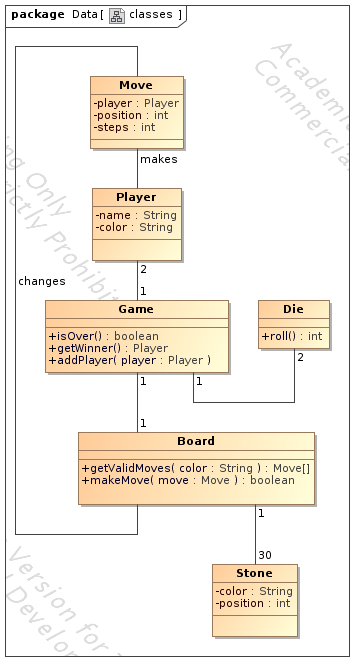
\includegraphics[scale=0.7]{classes.png}
\end{figure}
\newpage

\section{Requirements}

% Requirements
\textbf{Non-functional Requirements}
\begin{itemize}

\item the application should not take longer than a second to process user input and display the results:

\item the application should run on all operation systems that ruby 1.9.3 supports
\item the application must not crash on more than 1 \% user inputs
\item the application must be packaged as a ruby gem

\end{itemize}
\textbf{Functional Requirements}

\begin{itemize}
\item \emph{Application}
\begin{itemize}
\item on startup the game should ask for both players' names
\item the game must have a command-line interface
\item the game must declare a victor when a game has ended
\item the game must offer an option for rematch after the game has ended
\end{itemize}
\item \emph{Game rules}
\begin{itemize}
\item the game must randomly roll the dice to determine the starting player
\item the game must support all standard backgammon rules
\item the game must have a backgammon board with two rows of triangles in alternating color and each triangle is numbered 1-24 starting with the lower-right triangle.
\item the game must support representing stones of two colours - red and black
\item the game must start with a standard backgammon layout:
\begin{itemize}
\item 2 red stones on triangle 1
\item 5 red stones on triangle 12
\item 3 red stones on triangle 17
\item 5 red stones on triangle 19
\item 2 black stones on triangle 24
\item 5 black stones on triangle 13
\item 3 black stones on triangle 8
\item 5 black stones on triangle 6
\end{itemize}
\item the game must roll the dice for the player when it is player's turn.
\item valid moves are determined by the player's dice roll according to backgammon rules.
\end{itemize}
\item \emph{User interface}
\begin{itemize}
\item the user must see the following information at the beginning of his/her turn:
\begin{itemize}
\item the current board and stones layout
\item the outcome of the random dice roll
\item the list of valid moves for the player
\end{itemize}
\item the user must be able to input two positive integers in the form of "<triangle> <steps>" to move the topmost stone on the specified triangle by the specified amount of moves
\item the game must print out the declared victor when the game ends
\end{itemize}
\end{itemize}

\newpage

\section{Minutes from Meeting with Customer}

\hspace{1.5em}Customer: I have a couple of suggestions that could really improve GapBammon.\\
Firstly, there currently is no match system for keeping track of how many points a given player has gathered.
This brings us to another possible feature there is no doubling cube, which is a standard component of backgammon.
Additionally, we managed to find some bugs. Namely, the game ended up in an infinite loop.
   
The customer also pointed out some possible improvements to the user interface. The visual board could be improved to show stones that have been put on the bar and stones that have reached the basket. At the moment, users have to keep track by reading this information from lines below the board. 

Furthermore, the board is really basic and no way to easily differentiate between quadrants. This should definitely be fixed. 

\end{document}
